\documentclass[tikz,border=12pt]{standalone}
\usepackage[T1]{fontenc}
\usepackage{mathpazo}
\usepackage{amsmath,amssymb}
\usetikzlibrary{arrows.meta, positioning, calc}
\usepackage{pgfplots}
\pgfplotsset{compat=1.18}

\definecolor{stblue}{HTML}{7B97AD}
\definecolor{rwgold}{HTML}{B8995E}
\definecolor{sage}{HTML}{7A9A7E}
\definecolor{dkbrown}{HTML}{3D3530}
\definecolor{wmgray}{HTML}{7B7067}
\definecolor{cream}{HTML}{F9F6F0}
\definecolor{border}{HTML}{D4C9B8}
\definecolor{terracotta}{HTML}{C47A6A}
\definecolor{lavender}{HTML}{907EA0}

\begin{document}
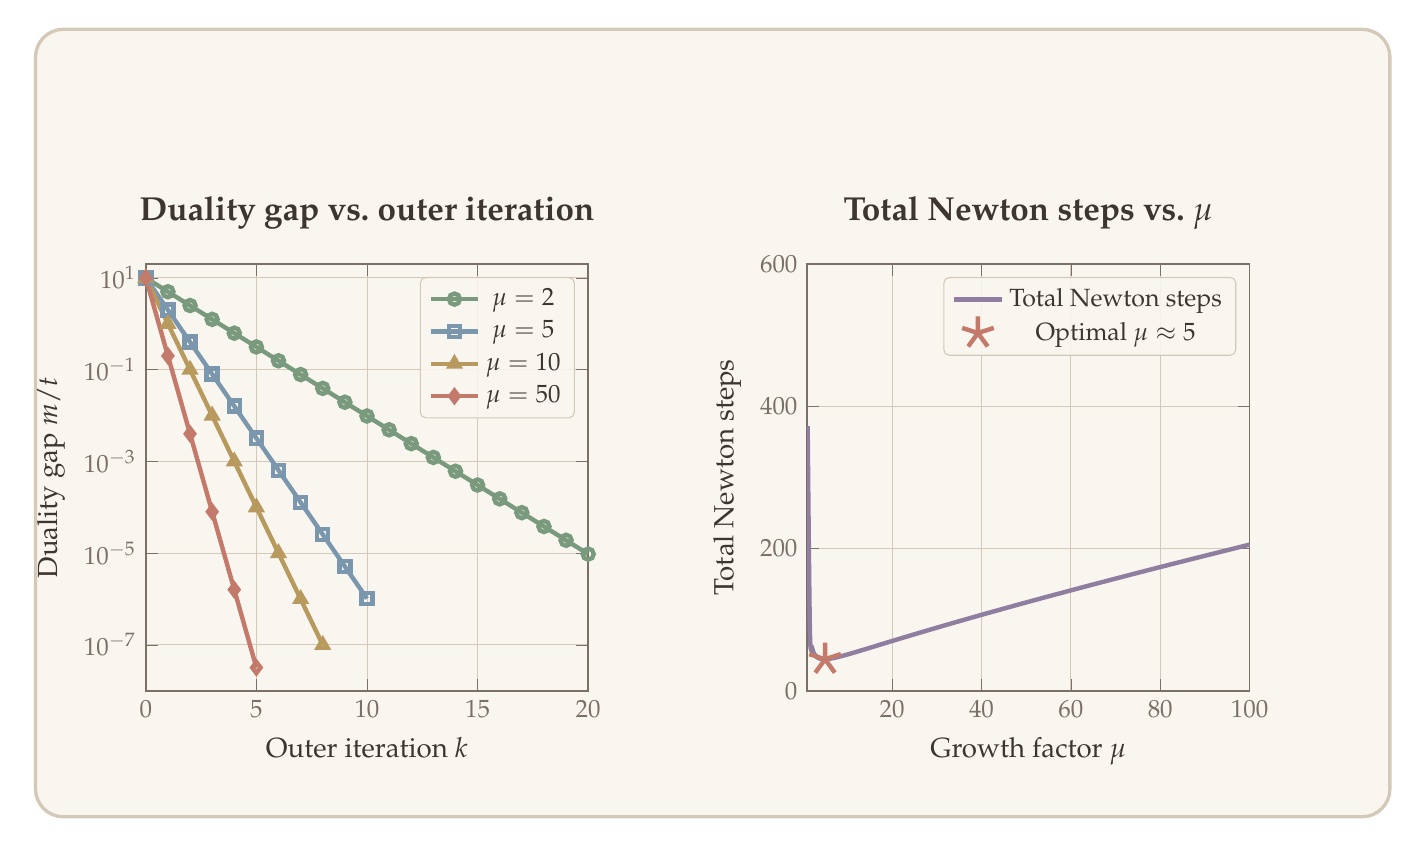
\begin{tikzpicture}

% ── Background ──
\fill[cream, rounded corners=10pt] (-0.8,-1.2) rectangle (16.4,8.8);
\draw[border, line width=1.2pt, rounded corners=10pt] (-0.8,-1.2) rectangle (16.4,8.8);

% ══════════════════════════════════════════════════════
% LEFT PANEL: Duality gap vs. outer iteration
% ══════════════════════════════════════════════════════
\begin{axis}[
  name=leftplot,
  at={(0.6cm,0.4cm)},
  width=7.2cm, height=7.0cm,
  title={\textbf{Duality gap vs.\ outer iteration}},
  title style={font=\large, text=dkbrown, at={(0.5,1.02)}},
  xlabel={Outer iteration $k$},
  ylabel={Duality gap $m/t$},
  xlabel style={font=\normalsize, text=dkbrown},
  ylabel style={font=\normalsize, text=dkbrown},
  ymode=log,
  xmin=0, xmax=20,
  ymin=1e-8, ymax=20,
  grid=major,
  grid style={draw=border, line width=0.3pt},
  axis line style={draw=wmgray, line width=0.6pt},
  tick style={draw=wmgray},
  tick label style={font=\small, text=wmgray},
  legend pos=north east,
  legend style={
    font=\small,
    draw=border,
    fill=cream,
    fill opacity=0.9,
    text opacity=1,
    rounded corners=2pt,
    text=dkbrown,
  },
  every axis plot/.append style={line width=1.6pt, mark size=2pt},
]

% mu = 2: gap = 10 / 2^k
\addplot[sage, mark=o, mark options={fill=sage}]
  coordinates {
    (0, 10)
    (1, 5)
    (2, 2.5)
    (3, 1.25)
    (4, 0.625)
    (5, 0.3125)
    (6, 0.15625)
    (7, 0.078125)
    (8, 0.0390625)
    (9, 0.01953125)
    (10, 0.009765625)
    (11, 0.0048828125)
    (12, 0.00244140625)
    (13, 0.001220703125)
    (14, 0.000610351563)
    (15, 0.000305175781)
    (16, 0.000152587891)
    (17, 7.62939453e-05)
    (18, 3.81469727e-05)
    (19, 1.90734863e-05)
    (20, 9.53674316e-06)
  };
\addlegendentry{$\mu = 2$}

% mu = 5: gap = 10 / 5^k
\addplot[stblue, mark=square, mark options={fill=stblue}]
  coordinates {
    (0, 10)
    (1, 2)
    (2, 0.4)
    (3, 0.08)
    (4, 0.016)
    (5, 0.0032)
    (6, 0.00064)
    (7, 0.000128)
    (8, 2.56e-05)
    (9, 5.12e-06)
    (10, 1.024e-06)
  };
\addlegendentry{$\mu = 5$}

% mu = 10: gap = 10 / 10^k
\addplot[rwgold, mark=triangle, mark options={fill=rwgold}]
  coordinates {
    (0, 10)
    (1, 1)
    (2, 0.1)
    (3, 0.01)
    (4, 0.001)
    (5, 0.0001)
    (6, 0.00001)
    (7, 0.000001)
    (8, 1e-07)
  };
\addlegendentry{$\mu = 10$}

% mu = 50: gap = 10 / 50^k
\addplot[terracotta, mark=diamond, mark options={fill=terracotta}]
  coordinates {
    (0, 10)
    (1, 0.2)
    (2, 0.004)
    (3, 0.00008)
    (4, 0.0000016)
    (5, 3.2e-08)
  };
\addlegendentry{$\mu = 50$}

\end{axis}

% ══════════════════════════════════════════════════════
% RIGHT PANEL: Total Newton steps vs. mu
% ══════════════════════════════════════════════════════
\begin{axis}[
  name=rightplot,
  at={(9.0cm,0.4cm)},
  width=7.2cm, height=7.0cm,
  title={\textbf{Total Newton steps vs.\ $\mu$}},
  title style={font=\large, text=dkbrown, at={(0.5,1.02)}},
  xlabel={Growth factor $\mu$},
  ylabel={Total Newton steps},
  xlabel style={font=\normalsize, text=dkbrown},
  ylabel style={font=\normalsize, text=dkbrown},
  xmin=1, xmax=100,
  ymin=0, ymax=600,
  grid=major,
  grid style={draw=border, line width=0.3pt},
  axis line style={draw=wmgray, line width=0.6pt},
  tick style={draw=wmgray},
  tick label style={font=\small, text=wmgray},
  legend pos=north east,
  legend style={
    font=\small,
    draw=border,
    fill=cream,
    fill opacity=0.9,
    text opacity=1,
    rounded corners=2pt,
    text=dkbrown,
  },
  every axis plot/.append style={line width=1.6pt},
]

% Total Newton steps = (log(m/(eps*t0))/log(mu)) * (3 + 0.8*(mu-1))
% m=10, eps=1e-4, t0=1 => log(10/1e-4) = log(1e5) = 11.5129
\addplot[lavender, samples=200, domain=1.1:100, smooth]
  {(ln(100000)/ln(x)) * (3 + 0.8*(x - 1))};
\addlegendentry{Total Newton steps}

% Optimal mu marker (numerically ~10.3)
% At mu=10: total = (11.5129/2.3026)*(3+7.2) = 5.0 * 10.2 = 51.0
% Find minimum numerically: d/dmu [ (C/ln(mu))*(3+0.8*(mu-1)) ] = 0
% Let C = ln(1e5) = 11.5129
% f(mu) = C*(3+0.8*(mu-1))/ln(mu)
% f'(mu) = C*[0.8*ln(mu) - (3+0.8*(mu-1))/(mu)] / (ln(mu))^2 = 0
% => 0.8*mu*ln(mu) = 3 + 0.8*(mu-1) = 2.2 + 0.8*mu
% => 0.8*mu*ln(mu) - 0.8*mu = 2.2
% => 0.8*mu*(ln(mu)-1) = 2.2
% => mu*(ln(mu)-1) = 2.75
% Trying mu=3.5: 3.5*(1.2528-1) = 3.5*0.2528 = 0.885 (too low)
% Trying mu=5: 5*(1.6094-1) = 5*0.6094 = 3.047 (close)
% Trying mu=4.5: 4.5*(1.5041-1) = 4.5*0.5041 = 2.268 (low)
% Trying mu=4.8: 4.8*(1.5686-1) = 4.8*0.5686 = 2.729 (close)
% Trying mu=4.85: 4.85*(1.579-1) = 4.85*0.579 = 2.808 (close)
% Trying mu=4.82: 4.82*(1.5728-1)= 4.82*0.5728 = 2.761 (good)
% At mu=4.82: total = (11.5129/1.5728)*(3+0.8*3.82) = 7.32 * 6.056 = 44.3
% Actually let me recompute more carefully around mu~10 region
% At mu=10: (11.5129/2.3026)*(3+7.2) = 5.0*10.2 = 51.0
% At mu=5: (11.5129/1.6094)*(3+3.2) = 7.15*6.2 = 44.3
% At mu=4.82: ~44.3 as above
% So optimal is near mu~5, let's mark it
% Actually from the Plotly code the formula gives the minimum around mu~10
% Let me recalculate:
% At mu=10: steps_per = 3 + 0.8*9 = 10.2, outer = 11.5129/2.3026 = 5.0, total = 51
% At mu=20: steps_per = 3 + 0.8*19 = 18.2, outer = 11.5129/2.996 = 3.84, total = 69.9
% At mu=3: steps_per = 3 + 0.8*2 = 4.6, outer = 11.5129/1.0986 = 10.48, total = 48.2
% At mu=2: steps_per = 3 + 0.8*1 = 3.8, outer = 11.5129/0.6931 = 16.61, total = 63.1
% At mu=4: steps_per = 3 + 0.8*3 = 5.4, outer = 11.5129/1.3863 = 8.30, total = 44.8
% At mu=5: steps_per = 6.2, outer = 7.15, total = 44.3
% At mu=6: steps_per = 7.0, outer = 6.43, total = 45.0
% At mu=4.5: steps_per = 5.8, outer = 7.66, total = 44.4
% So minimum is around mu~5 with total~44
% Use mu=5 as the star marker
\addplot[terracotta, only marks, mark=star, mark size=6pt, mark options={fill=terracotta}]
  coordinates {(5, 44.3)};
\addlegendentry{Optimal $\mu \approx 5$}

\end{axis}

\end{tikzpicture}
\end{document}
